% Created 2018-11-22 tor 17:54
% Intended LaTeX compiler: pdflatex
\documentclass[11pt]{article}
\usepackage[utf8]{inputenc}
\usepackage[T1]{fontenc}
\usepackage{graphicx}
\usepackage{grffile}
\usepackage{longtable}
\usepackage{wrapfig}
\usepackage{rotating}
\usepackage[normalem]{ulem}
\usepackage{amsmath}
\usepackage{textcomp}
\usepackage{amssymb}
\usepackage{capt-of}
\usepackage{hyperref}
\newcommand{\lo}[1]{\underline{#1}}
\newcommand{\hi}[1]{\overline{#1}}
\author{Joel Dahne}
\date{\today}
\title{SwapMob: Swapping trajectories for mobility Data anonymization}
\hypersetup{
 pdfauthor={Joel Dahne},
 pdftitle={SwapMob: Swapping trajectories for mobility Data anonymization},
 pdfkeywords={},
 pdfsubject={},
 pdfcreator={Emacs 25.2.2 (Org mode 9.1.14)},
 pdflang={English}}
\begin{document}

\maketitle
\tableofcontents


\section{Define trajectories and co-trajectories}
\label{sec:org7a8c28a}
We begin by defining what we mean with trajectories and
co-trajectories.

Informally, a trajectory is a number of measurements of location
together with the times for the measurements. An example would be
position data from a GPS taken at certain times. Let \(L\) be the
location space consisting of all possible measurements of location,
this could for example be the set of GPS coordinates or the set of
coordinates on a city map. A measurement is given by a location
together with a timestamp, i.e. a measurement \(m\) can be represented
by an element in the set \(L \times \mathbb{R}\). We can now define a
trajectory as a set of measurements, a trajectory, \(r\), is then
given by a subset of \(L \times \mathbb{R}\). Let us denote the set of
trajectories by \(T\).

\textbf{Remarks:} Here we have a couple of options. We could choose to allow
at most one measurement per timestamp, i.e. for a trajectory, \(r\),
there is no time \(t\) such that we have two measurements at that
time, \((x_1, t)\) and \((x_2, t)\), with \(x_1 \not= x_2\). At first
I believe this makes sense, you can't be in two different places at
the same time, but depending on the resolution we have for the time
this might happen, for example this is the case for the CDR data.
Another thing is that defining \(r\) as a subset of \(L \times
\mathbb{R}\) does not allow for duplicate measurements, i.e. two
measurements at the same time with the same location, I don't believe
this is a problem, we can simply remove any duplicates from the data
set. One benefit of having trajectories as sets is that it is easy to
talk about the union and intersection of several trajectories. One
drawback of not allowing multiple measurements at the same time would
be that the union of two trajectories might not be a trajectory. One
important thing to note is that we do not have any information about
an individual with this definition, trajectories are fully anonymous,
instead we encode the data about individuals in the co-trajectory.

With a co-trajectory we mean a number of trajectories that each
correspond to some, possible anonymized, individual. Let \(I\) be the
set of individuals, we can define a co-trajectory, \(R\) by a function
from \(I\) to \(T\). That is, a co-trajectory is given by a function
\(R: I \to T\) and the trajectory of an individual \(\iota \in I\) is
then given by the trajectory \(R(\iota) \in T\).

\textbf{Remarks:} One benefit of defining a co-trajectory as a function is
 that we get a natural way of talking about the trajectories of
 individuals. It also becomes easy to talk about sets of trajectories,
 for example \(R(I)\) is the set of trajectories for all the
 individuals. With \(R\) being a function we need to give trajectories
 for all individuals in \(I\), but if there is any individual we don't
 have any data for we can just give it the empty trajectory,
 \(R(\iota) = {\emptyset}\).
\section{Define a swap}
\label{sec:orge90c233}
We first define what we mean with a swap of two trajectories and then
what we mean with a \texttt{valid} swap.

Let \(r_1\) and \(r_2\) be two trajectories. Swapping \(r_1\) and
\(r_2\) at times \(t_1\) and \(t_2\) gives two new trajectories,
\(\overline{r_1}\) and \(\overline{r_2}\) given by
\begin{equation}
  \overline{r_1} = \{(x, t) \in r_1: t < t_1\} \cup \{(x, t) \in r_2: t \geq t_2\}
\end{equation}
and
\begin{equation}
  \overline{r_2} = \{(x, t) \in r_2: t < t_2\} \cup \{(x, t) \in r_1: t \geq t_1\}.
\end{equation}
Formally we can see it as a function \(\textrm{swap}: T \times T
\times \matbb{R} \times \mathbb{R} \to T \times T\) with
\begin{equation}
  \textrm{swap}(r_1, r_2, t_1, t_2) = (\overline{r_1}, \overline{r_2}).
\end{equation}

\textbf{Remarks:} We here have no requirements on which trajectories can be
swapped and at what times. It is basically just taking two
trajectories and swapping parts of their path. Note that the times
\(t_1\) and \(t_2\) doesn't even have to occur in the two
trajectories.

To define which swaps are \texttt{valid} we first define what we mean with
two measurements being \texttt{similar}. Two measurements \((x_1, t_1)\) and
\((x_2, t_2)\), are similar if \(d(x_1, x_2) \leq \chi\) and \(|t_1 -
t_2| \leq \tau\), we denote this by \((x_1, t_1) \approx (x_2, t_2)\).
From this we can say that two trajectories meet if they have
measurements which are similar. More precisely \(r_1\) and \(r_2\)
meet at time \((t_1, t_2)\) if there exists \((x_1, t_1) \in r_1\) and
\((x_2, t_2) \in r_2\) such that \((x_1, t_1) \approx (x_2, t_2)\), we
denote this by \(r_1 \approx_{(t_1, t_2)} r_2\).

\textbf{Remarks:} The notion of two measurements being similar depends on
\(\chi\) and \(\tau\) and they need to be chosen with respect to the
accuracy of the data. Two trajectories can meet several times and one
measurement can be involved in several meetings.

A swap of \(r_1\) and \(r_2\) at time \((t_1, t_2)\) is \texttt{valid} if
\(r_1 \approx_{(t_1, t_2)} r_2\).

\textbf{Remarks:} With this definition a swap can only be valid if the exact
times for the swap occur in the measurements, for a general swap this
was not required.
\section{Swaps on co-trajectories}
\label{sec:org1bcd558}
A swap on a co-trajectory \(R\) is given by a pair of ids, the
trajectories to swap, and a pair of times, \((t_1, t_2)\), with the
times for the swap. Formally a swap is thus defined by an element from
the set \(I \times I \times \mathbb{R} \times \mathbb{R}\). The notion
of a \texttt{valid} swap is the same as before, the swap \((\iota_1, \iota_2,
t_1, t_2)\) is valid if \(R(\iota_1) \approx_{(t_1, t_2)}
R(\iota_2)\). We can also add the requirement that the ids should be
different. We can see it as a function \(\textrm{swap}: (I \to L
\times \mathbb{R}) \times I \times I \times \mathbb{R} \times
\mathbb{R} \to (I \to L \times \mathbb{R})\).

\textbf{Remarks:} The main problem with this definition is that the swap
given by \((\iota_1, \iota_2, t_1, t_2)\) is different from the swap
given by \((\iota_2, \iota_1, t_2, t_1)\) even though we would like
them to be the same. One way to solve this is to consider the
equivalence relation where two swaps are equivalent if and only if
they are on this form.

We can talk about the set of all swaps for a co-trajectory, with this
we mean the set \((I \times I \times \mathbb{R} \times
\mathbb{R})/\sim\) where \(\sim\) is the equivalence relation from the
above remark. A subset of the set of all swaps is the set of all
\texttt{valid} swaps, which we, for a co-trajectory \(R\), will denote by
\(S(R))\).

\textbf{Remarks:} With this all elements of \(S(R))\) are valid swaps and it
 does not contain duplicate swaps nor does it contain swaps of a
 trajectory with itself (because the latter are not valid swaps).

Given \(S(R)\) we want to perform some or all of these swaps on \(R\).
The problem here is that \(S(R)\) is not stable under swaps. Let \(s
\in S(R)\) be a swap and \(R' = \textrm{swap(R, s)}\) denote the
co-trajectory after performing the swap. In general we do not have
\(S(R) = S(R')\). Two things can happen, the ids of the possible swaps
can change or swaps that were not valid become valid or the other way
around.
\subsection{Example when ids swap}
\label{sec:orgff9a4e3}
Consider the co-trajectory \(R\) given by \(I = \{\iota_1, \iota_2,
\iota_3}\) and
\begin{align}
  R(\iota_1) &= \{((0, 1), 0), ((1, 1), 1), ((2, 1), 2)\}\\
  R(\iota_2) &= \{((0, 2), 1), ((1, 2), 2), ((2, 2), 3)\}\\
  R(\iota_3) &= \{((1.05, 0), 0), ((1.05, 1), 1), ((1.05, 2), 2), ((1.05, 3), 3)\}\\
\end{align}
It has \(S(R) = \{(\iota_1, \iota_3, 1, 1), (\iota_2, \iota_3, 2,
2)\}\).

After performing the swap given by \((\iota_1, \iota_3, 1, 1)\) we get
the co-trajectory \(R'\) and now have \(S(R') = \{(\iota_1, \iota_3,
1, 1), (\iota_2, \iota_1, 2, 2)\}\). In particular \(S(R) \not=
S(R')\). See Figure \ref{fig:org751ffd7}.

Essentially it is the same measurements which participate in the swaps
for \(S(R)\) and \(S(R')\) but they belong to different ids.
\begin{figure}[htbp]
\centering
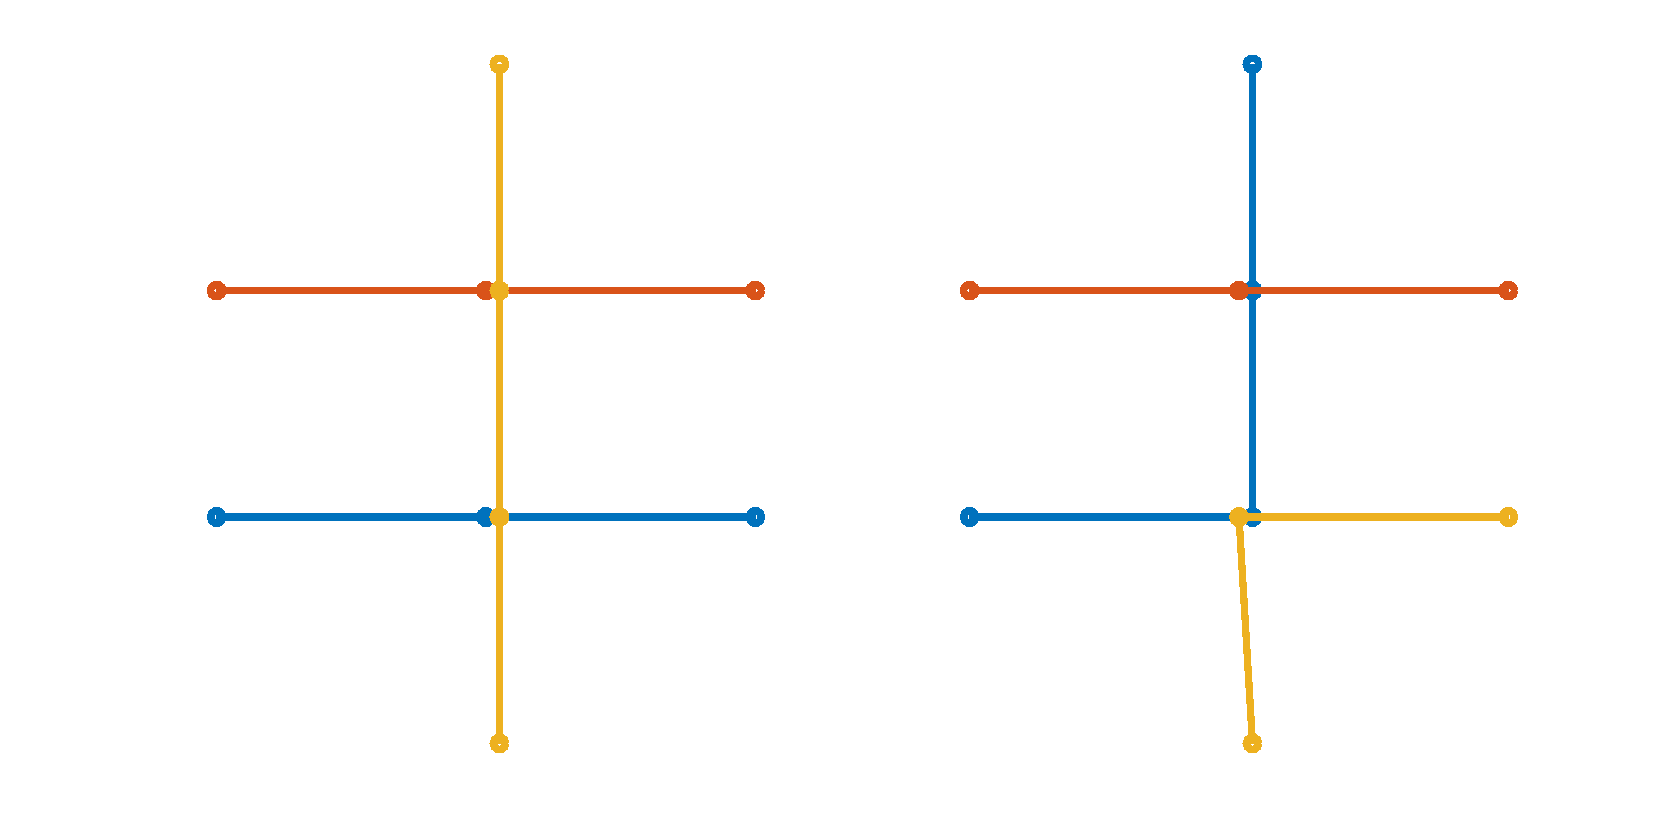
\includegraphics[width=.9\linewidth]{./figures/swap-ids.pdf}
\caption{\label{fig:org751ffd7}
The co-trajectories \(R\) and \(R'\). The ids in \(S(R)\) and \(S(R')\) are different.}
\end{figure}
\subsection{Example when which swaps are valid change.}
\label{sec:org3b1bf91}
Consider the co-trajectory \(R\) given by \(I = \{\iota_1, \iota_2\}\)
and
\begin{align}
  R(\iota_1) &= \{((1.1, 0), 0), ((1.1, 1), 1), ((1, 1), 1.05), ((0, 1), 2)\}\\
  R(\iota_2) &= \{((1.05, 2), 0), ((1.1, 1.1), 1), ((2, 1.1), 2)\}\\
\end{align}
It has \(S(R) = \{(\iota_1, \iota_2, 1, 1), (\iota_1, \iota_2, 1.05,
1)\}\).

After performing the swap given by \((\iota_1, \iota_2, 1, 1)\) we get
the co-trajectory \(R'\) and now have \(S(R') = \{(\iota_1, \iota_2,
1, 1), (\iota_1, \iota_2, 1, 1.05)\}\). In particular \(S(R) \not=
S(R')\). See figure \ref{fig:org2db6100}.

Here the measurements that participates in the swaps has changed. In
the beginning the two measurements \(((1.1, 1), 1)\) and \(((1, 1),
1.05)\) were in the same trajectory and could not be used for a swap.
But after the first swap they are no longer in the same trajectory and
can now be used for a swap. Similarly, for the two measurements \(((1,
1), 1.05)\) and \(((1.1, 1.1), 1)\) could swap in the beginning but
after the first swap they are in the same trajectory and can't swap
anymore.
\begin{figure}[htbp]
\centering
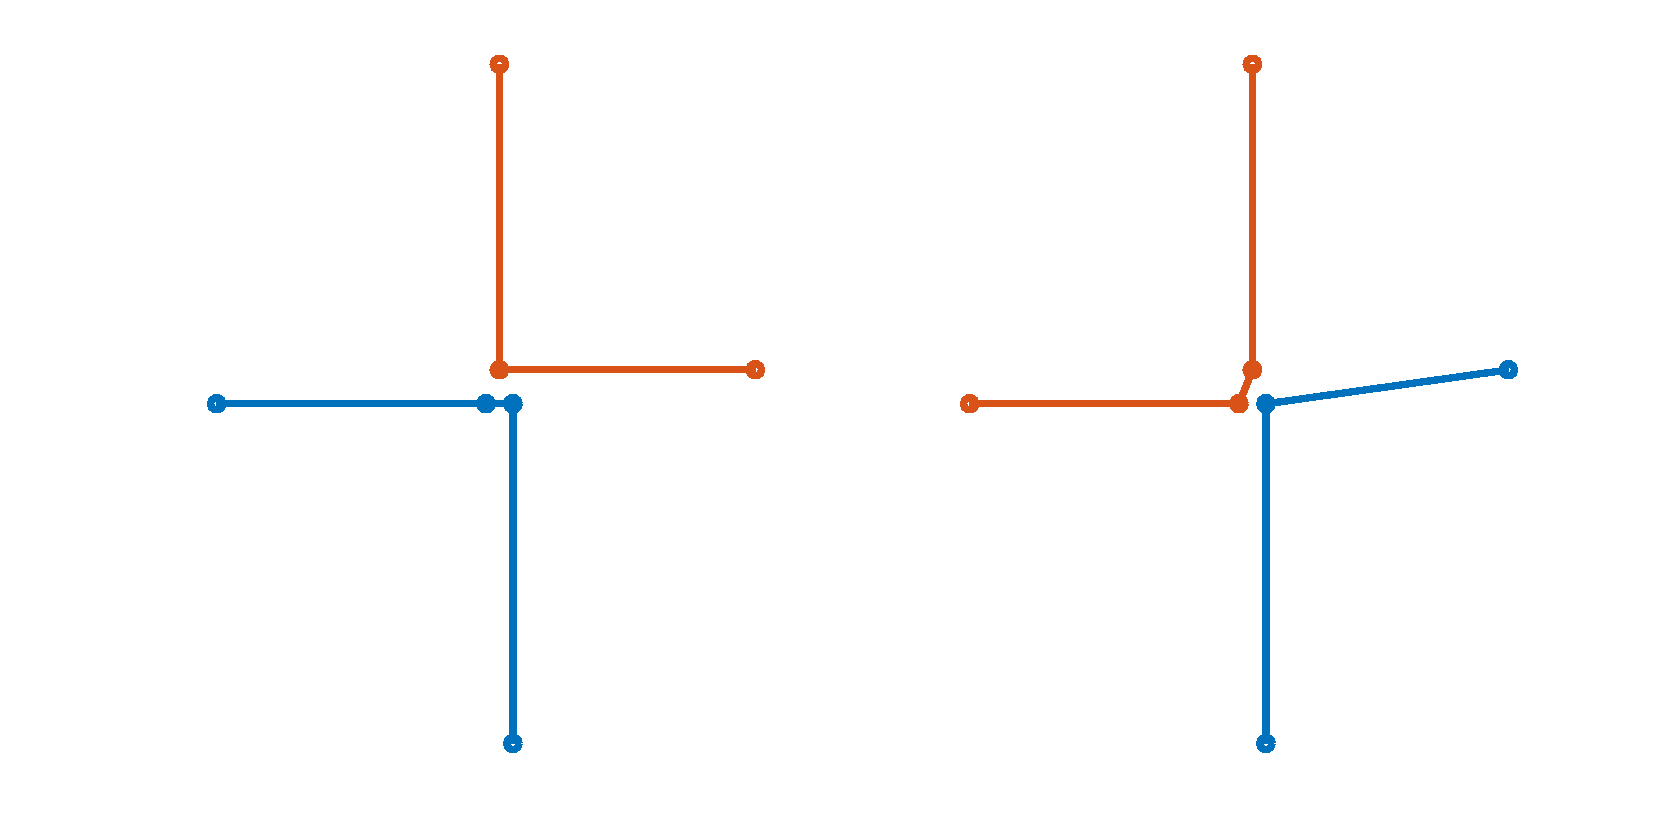
\includegraphics[width=.9\linewidth]{./figures/swap-valid.pdf}
\caption{\label{fig:org2db6100}
The co-trajectories \(R\) and \(R'\). The measurments that are valid for swaps are different for \(R\) and \(R'\).}
\end{figure}
\subsection{Handling multiple swaps}
\label{sec:org24af9d0}
As seen the set of valid swaps for a co-trajectory can change when we
apply swaps to it. This means that we have no natural definition of
\texttt{applying all possible swaps} to a co-trajectory. For example one
natural thing to do would be to take the set of all valid swaps and
choose an order of them, we them perform the swaps in the given order.
The problem with this would then be that after performing the first
swap the second one might no longer be valid and there could also be
other swaps that become valid as we perform swaps.

How can we solve this? The type of problem occurring in example 1
above can be solved in a fairly natural way by, every time we perform
a swap also swap the ids of the relevant swaps in the list of swaps we
want to perform. Let \(S\) be the set of swaps we want to perform,
pick one \(s = (\iota_1, \iota_2, t_1, t_2) \in S\) and perform that
swap on the co-trajectory. After this the swaps in \(S\) might no
longer be valid swaps for the new co-trajectory, we can fix this by
replacing all swaps on the form \((\iota_1, \iota, t'_1, t),\ t'_1
\geq t_1\) in \(S\) with \((\iota_2, \iota, t'_1, t)\) and similar for
swaps on the form
\begin{align}
  (\iota, \iota_1, t, t'_1), & \ t'_1 \geq t_1,\\
  (\iota_2, \iota, t'_2, t), & \ t'_2 \geq t_2,\\
  (\iota, \iota_2, t, t'_2), & \ t'_2 \geq t_2.
\end{align}
What we are using here is essentially that the measurements which are
valid to use for swaps remain the same, the only difference being that
they might have swapped ids.

The type of problem occurring in the second example is harder to
handle. It would require us to remove and insert swaps in the list of
swaps we want to perform after every swap. Then we get a problem of
knowing which swaps have already been performed. In the previous case
we had a number of swaps in the beginning and then we only needed to
update some ids to keep them valid, it is fairly easy to keep track of
which swaps have been performed. I'm still not sure how to handle
this. The problem comes from the fact that we do not allow
trajectories to swap with themselves. If we allow trajectories to swap
with themselves this problem goes away, then the size of \(S(R)\) will
stay constant under swaps and only the ids will change. I believe this
would be the most natural solution to the problem but I'll have to
think more about the consequences.
\subsection{Order of swaps}
\label{sec:org2cd5463}
The order of the swaps matter. For example consider the co-trajectory
\(R\) given by \(I = \{\iota_1, \iota_2, \iota_3\}\) and
\begin{align}
  R(\iota_1) &= \{((0, 0), 0), ((1, 0.95), 1), ((2, 0), 2)\}\\
  R(\iota_2) &= \{((0, 1), 0), ((1, 1.00), 1), ((2, 1), 2)\}\\
  R(\iota_3) &= \{((0, 2), 0), ((1, 1.05), 2), ((2, 2), 2)\}\\
\end{align}
It has \(S(R) = \{s_1, s_2, s_3\} = \{(\iota_1, \iota_2, 1, 1),
(\iota_1, \iota_3, 1, 1), (\iota_2, \iota_3, 1, 1)\}\).

There are six different orders to perform the swaps in, we'll show
that at least two of them are different. First consider the order
\(s_1 \to s_2 \to s_3\), it gives the result seen in Figure
\ref{fig:orga235c8f}. Performing the swaps in the order \(s_2 \to s_1 \to
s_3\) gives us the result in Figure \ref{fig:orgae8e0e5}. We can see that
the results are not the same.
\begin{figure}[htbp]
\centering
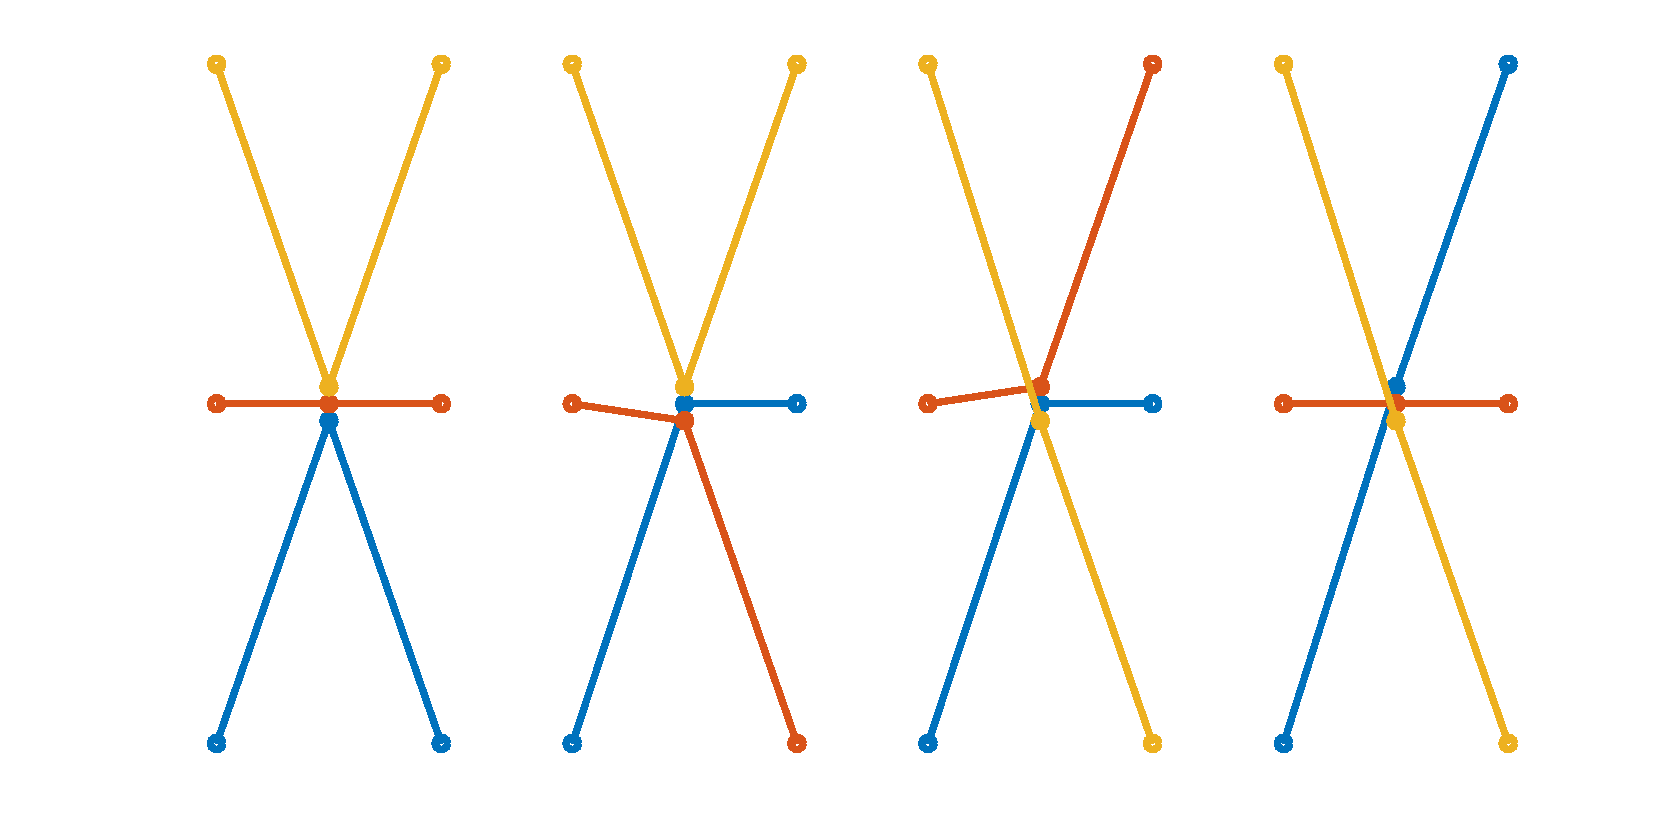
\includegraphics[width=.9\linewidth]{figures/swap-order-1.pdf}
\caption{\label{fig:orga235c8f}
Changes of the co-trajectory \(R\) when performing the swaps in the order \(s_1 \to s_2 \to s_3\).}
\end{figure}

\begin{figure}[htbp]
\centering
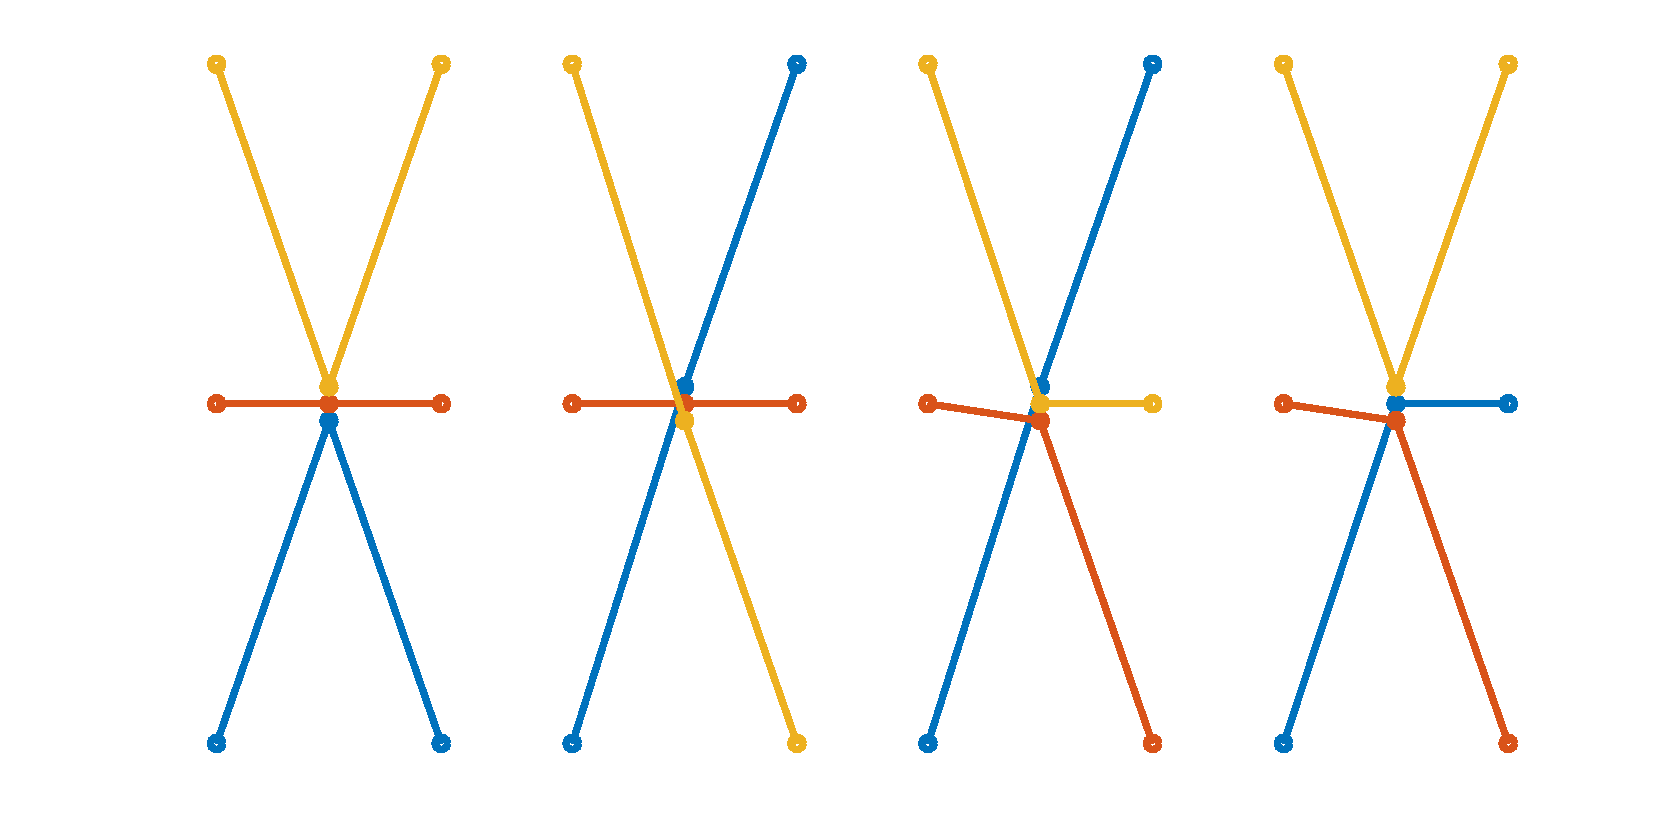
\includegraphics[width=.9\linewidth]{figures/swap-order-2.pdf}
\caption{\label{fig:orgae8e0e5}
Changes of the co-trajectory \(R\) when performing the swaps in the order \(s_2 \to s_1 \to s_3\).}
\end{figure}

Since the order of the swap matters we need to choose on to use, the
most natural thing is probably to take a random order.
\section{Give a complete algorithm}
\label{sec:org6f941d9}
Following the discussions above a possible implementation would be to
first compute all possible swaps, including individuals swapping with
themselves. We then randomly choose and order to perform the swaps in.
When performing a swap we first check if it is a swap with itself, if
so we do nothing, otherwise randomly choose if we should apply the
swap or not. If we applied the swap we update the ids of all coming
swaps that they are still valid. We finish when we have gone through
all the swaps.

A Python implementation of the algorithm is given below.
\begin{verbatim}
import numpy as np
import matplotlib.pyplot as plt
import random

## Trajectory r = [((x, y), t)]
## Individuals i = int
## Co-trajectory R = dict(individual, trajectory)
## Swap s = (i_1, i_2, t_1, t_2)

def swapTrajectories(r1, r2, t1, t2):
    """Swap the two trajectories r1 and r2 at time (t1, t2)."""
    r1p = ([(l, t) for (l, t) in r1 if t < t1]
           + [(l, t) for (l, t) in r2 if t >= t2])
    r2p = ([(l, t) for (l, t) in r2 if t < t2]
           + [(l, t) for (l, t) in r1 if t >= t1])
    return r1p, r2p

def swap(R, s):
    """Perform the swap given by s on the co-trajectory R."""
    Rp = R.copy()
    Rp[s[0]], Rp[s[1]] = swapTrajectories(R[s[0]], R[s[1]], s[2], s[3])
    return Rp

def updateSwaps(S, s):
    """Update the set of swaps S so that they are all valid after
    performing the swap s.
    """
    Sp = set()
    for sp in S:
        # Check if the first id is equal to one of the swapped ones
        # and the time is later than the swapped time, if so swap it
        if (sp[0] == s[0] and sp[2] >= s[2]):
            sp = (s[1], sp[1], sp[2], sp[3])
        elif (sp[0] == s[1] and sp[2] >= s[3]):
            sp = (s[0], sp[1], sp[2], sp[3])

        # Check if the second id is equal to one of the swapped ones
        # and the time is later than the swapped time, if so swap it
        if (sp[1] == s[0] and sp[3] >= s[2]):
            sp = (sp[0], s[1], sp[2], sp[3])
        elif (sp[1] == s[1] and sp[3] >= s[3]):
            sp = (sp[0], s[0], sp[2], sp[3])

        Sp.add(sp)

    return Sp

def dist(x1, x2):
    """Returns the distance between x1 and x2."""
    return math.sqrt((x1[0] - x2[0])**2 + (x1[1] - x2[1])**2)

## Hard coded values for chi and tau
chi = 0.1
tau = 0.1

def similar(m1, m2):
    """Returns true if the measurements m1 and m2 are similar."""
    if m1 == m2:
        return False

    if dist(m1[0], m2[0]) <= chi and abs(m1[1] - m2[1]) <= tau:
        return True

    return False

def swapsTrajectories(r1, r2, i1=None, i2=None):
    """Return the set of all valid swaps between the two trajectories r1
    and r2. If two ids are given, add these two to the swaps.
    """
    S = set()
    for m1 in r1:
        for m2 in r2:
            if similar(m1, m2):
                if i1 == None and i2 == None:
                    S.add((m1[1], m2[1]))
                else:
                    S.add((i1, i2, m1[1], m2[1]))
    return S

def swaps(R):
    """Return the set of all valid swaps on R."""
    S = set()
    for i1 in R:
        for i2 in R:
            if i1 <= i2:
                S.update(swapsTrajectories(R[i1], R[i2], i1, i2))

    return S

def SwapMob(R):
    S = swaps(R)
    while len(S) > 0:
        ## Pick a random swap to perform
        s = S.pop()
        ## Check so that it is not a swap with itself
        if s[0] != s[1]:
            ## Randomly choose to apply the swap or not
            if random.choice([True, False]):
                R = swap(R, s)
                S = updateSwaps(S, s)

    return R

## Methods for plotting co-trajectories
def plotTrajectory(r):
    r = sorted(r, key=lambda m: m[1])
    plt.plot(list(map(lambda m: m[0][0], r)),
             list(map(lambda m: m[0][1], r)), "o-")

def plotCoTrajectory(R):
    for i in R:
        plotTrajectory(R[i])
\end{verbatim}

\textbf{Remarks:} The reason not to allow an individual to swap with itself
 is that it is not well defined what the new trajectory will be, we
 can give in two identical trajectories to the swap function but it
 will give out two different ones and we would have to choose one to
 use. The reason that will still allow swaps where individual swap
 with themselves is that when we get to that swap it might no longer
 be a swap with itself because we change the ids when updating swaps
 in every step. The implementation above is in no way optimized, I
 believe it has quadratic complexity which is probably not feasible
 for larger datasets.
\section{Privacy gains vs utility}
\label{sec:org2e4e918}
What kind of privacy gains can we expect from \texttt{SwapMob}? I think it
depends a lot on what we assume about how trajectories of individuals
behave.

To begin with, what are we comparing with? We get the least amount of
privacy if we just publish the original co-trajectory with,
anonymized, individuals and their trajectories. On the other end I
would say that we have just publishing the measurements with no data
about individuals whatsoever. You could consider even more drastic
things, like not publishing any data at all, perturbing measurements
or removing/adding measurements/trajectories. I do however think that
it is somewhat natural to not touch the measurements and only the
individuals data and I'll therefore compare to publishing all data or
publishing only measurements.

Swapping trajectories can never give more privacy than only publishing
measurements. We therefore have to consider if publishing only
measurements preserves enough privacy for our use case, if that is not
the case swapping trajectories can never solve the problem. Assume
that we would be okay with publishing only measurements, the reason to
instead publish swapped trajectories would be that it keeps more of
the utility of the data but still might preserve enough privacy. What
we want to do is therefore to compare the amount of preserved privacy
between publishing all data and publishing swapped data and also
compare the utility from publishing only measurements to publishing
swapped data.

\subsection{Utility}
\label{sec:orge9608d0}
I do not yet know enough to be able to compare utility for different
kinds of data. The reason is that I don't know what kind of analysis
you in general want to do with the data. We can look at different
metrics of the data and see which ones are preserved when we swap
trajectories or which ones only depend on the measurements and not on
which individual they belong to. But to do this I would need to know
which kinds of metrics are interesting.

\subsection{Privacy}
\label{sec:orgd5206f0}
I'll here give a couple of thoughts and ideas without much detail and
with no attempts of proofs.

The idea of \texttt{SwapMob} is that if an adversary is able to identify an
individual with part of a trajectory it only learns the moment of the
individual up until the next possible swap for that trajectory. But to
what extent is this true? To answer this question we need to do some
assumptions about the distribution of trajectories.

Assume that trajectories are Markov processes, given a point on a
trajectory you only need the information about the location and time
of that measurement to know the probability distribution of the next
point on the trajectory. In other words the movement of an individual
only depends on the current position and time and not on prior
movement. In this case I believe \texttt{SwapMob} works as intended. If an
adversary has identified parts of a trajectory that belongs to an
individual it can follow the trajectory of the individual up until the
next time it crosses another trajectory. With the assumption that
trajectories are Markov processes the adversary will not be able to
figure out if a swap occurred or not, it can only guess with a 50/50
chance of being correct. \textbf{Prove this}

If trajectories are not Markov processes but instead the movement of
an individual depends on the historic movement, \texttt{SwapMob} will not
work as well. For example assume that if an individual has been moving
in a straight line for some time the probability of it continuing in a
straight line is high. Consider the case of two trajectories going in
opposite directions meeting. If we swap these we would get two
trajectories that go in a straight line and then both turn around
completely at the same time. This scenario would be much more unlikely
than the case of both just continuing in a straight line, so if the
adversary sees this happening it can guess that a swap occurred here
and be correct with a high probability. \textbf{Formalise this}
\section{Alternatives}
\label{sec:orgdac8846}
\subsection{Distance vs grid}
\label{sec:org4b35a4e}
As mentioned above we call two measurements, \((x_1, t_1)\), \((x_2,
t_2)\), similar if \(d(x_1, x_2) \leq \chi\) and \(|t_1 - t_2| \leq
\tau\). We can say that this uses distance to determine if two
measurements are similar or not.

Another approach would be to use a grid to determine similarity. To do
that we split \(L\) into subsets that are all disjoint and whose union
is equal to \(L\). We also split \(\mathbb{R}\) into half open
intervals that are also disjoint and cover the whole line. Two
measurements, \((x_1, t_1)\), \((x_2, t_2)\), are now similar if
\(x_1\) and \(x_2\) lie in the same subset of \(L\) and \(t_1\) and
\(t_2\) lie in the same interval. If \(L = \mathbb{R}^2\) a simple
example would be to have the grid given by the points with integer
coordinates, with \(b_{i,j} = [i, i+1) \times [j, j+1)\) \(L\) is
given by
\begin{equation}
  L = \bigcup_{i, j = -\infty}^\infty b_{i,j}
\end{equation}
and in the same way let \(\tau_i = [i, i+1)\) and we get
\begin{equation}
  \mathbb{R} = \bigcup_{i = -\infty}^\infty \tau_i.
\end{equation}
Then two measurements \(((x_1, y_1), t_1)\) and \(((x_2, y_2), t_2)\)
are similar if \((x_1, y_1)\) and \((x_2, y_2)\) lie in the same
\(b_{i,j}\) and \(t_1\) and \(t_2\) lie in the same \(\tau_i\).

One drawback of the grid approach is that if two measurements are very
close two the boundaries in the grid they can be very close to each
other but still not be considered similar since they are in different
boxes.

The grid approach does however come with several benefits. One big
benefit is that the relation \texttt{being similar} becomes transitive and
thus also an equivalence relation, this should make some things easier
to work with. I also believe it should make it easier to do an
efficient implementation.

The article first uses the distance definition when introducing
similarity for measurements In the pseudo algorithm it uses grids for
the time stamp but distance for the position. Finally I believe the R
code uses a grid approach for both time and position.
\subsection{Strict or not strict inequalities}
\label{sec:orgc398e40}
There are a number of inequalities occurring in the definitions and we
have to choose which ones to make strict and which ones should not be
strict.
\subsubsection{Swapping}
\label{sec:orga86a350}
When swapping two trajectories \(r_1\) and \(r_2\) at time \(t_1\) and
\(t_2\) we have to choose what happens with measurements occurring
exactly at time \(t_1\) or \(t_2\). In the above definitions I have
chosen to swap measurements occurring exactly at these times, though
that choice was fairly random and I'm not sure that is the optimal
choice.

One reason for not swapping those measurements would be that the proof
for privacy preservation assuming trajectories are Markov chains
becomes easier, at least I believe this is the case.
\subsubsection{Similarity}
\label{sec:org9bb01f9}
When defining what is means for two measurements to be \texttt{similar} I
have not used strict inequalities. In this case I believe this is the
only valid option since we otherwise have no way of requiring exact
equality (putting \(\chi\) or \(\tau\) to zero) which could make sense
in some cases, in particular in a discrete setting.
\section{Swaps using grids}
\label{sec:org115e117}
Above we discussed using grids as an alternative to distance for
defining similarity of measurements and swaps. We here give a formal
definition of this and also an algorithm for it.

We keep the same definitions for trajectories and co-trajectories but
we redefine what it means for two measurements to be \texttt{similar} and
when a swap is \texttt{valid}. Most definitions come naturally but we have to
take care of some edge cases.
\subsection{Grid}
\label{sec:orgd853a50}
With a grid we mean a partition of a set into disjoint subsets. In
general we'll refer to it simply as a partition and not as a grid.

For time we'll always use a partition consisting of half open
intervals of the same size covering the real line, given \(\tau \in
\mathbb{R}\) we have the partition given by
\begin{equation}
  \mathbb{R} = \bigcup_{i=-\infty}^\infty [i\tau, (i+1)\tau)
\end{equation}
and we'll use the notation \(\tau_i = [i\tau, (i+1)\tau)\). The choice
of \(\tau\) depends on the particular problem.

For \(L\) the partitioning will depend both on the precise choice of
\(L\) and also on the current problem. The general notation we'll use
is that \(L\) is partitioned into the sets \(\{\chi_i\}_{i \in I}\)
for some index set \(I\) with \(\chi_i \subset L\) and \(\chi_i \cap
\chi_j = \emptyset\) if \(i \not= j\) and so that we have
\begin{equation}
  L = \bigcup_{i \in I} \chi_i.
\end{equation}
In general we think of the subsets \(\chi_i\) as connected and fairly
regular. For example if \(L = \mathbb{R}^n\) a natural partitioning is
into half open boxes of the same size. If \(L\) is a graph we could
partition it into its nodes. Another example would be to have \(L\) be
given by a compact subset of \(\mathbb{R}^2\) representing a map of
some city or other geographical area, then it could be natural to
choose the partition using its geographic properties, partitioning it
into parts bounded by rivers, mountains or similar.

\textbf{Remarks:} The precise choice of the partition is highly dependent on
the problem. How fine the partitions should be depends on how often
measurements are taken and how precise the measured location is. In
cases when the precision of the measurements are not uniform over
\(L\) it might be natural to choose a nonuniform partition over \(L\),
this would for example be the case with data from cell phones where
the precision depends on number of cell towers in the area.
\subsection{Similarity}
\label{sec:orgba7eda7}
With the above definitions of a partition the definition of similarity
for measurements become very simple. Two measurements \((x_1, t_1)\)
and \((x_2, t_2)\) are similar if \(x_1\) and \(x_2\) belong to the
same part \(\chi_i\) and \(t_1\) and \(t_2\) belong to the same part
\(\tau_i\).

This gives some important differences compared to defining similarity
based on distance between measurements. The most important difference
is that \texttt{being similar} becomes an equivalence relation on \(L \times
\mathbb{R}\), what was missing before was the transitivity. Having an
equivalence relation comes with a number of benefits, as we'll see
below.
\subsection{Swaps}
\label{sec:org1552201}
We could define a swap to be \texttt{valid} in exactly the same way as before
only using the new notion of similarity. With the grid approach we do
however have some more options and we'll use a slightly different
approach.

To begin with, since similarity is now an equivalence relation it will
partition the set of measurements into groups where all measurements
are similar to each other. It then makes sense to define swapping on
these groups of measurements instead of only pairwise, as we did
before.

We begin by considering only the case when every trajectory has at
most one measurement for each time partition \(\tau_i\), in this case
the natural and simple. After that we'll consider the case with the
trajectories possibly having several measurements in a time partition.
We'll see that we have a couple of different options with what to do
then, all of them coming with some problems.

Now, assume that the measurements \(m_1, m_2, \dots, m_n\) belonging
to the trajectories \(r_1, r_2, \dots, r_n\) all are similar and lie
in the set \(\chi_i \times \tau_j\). Further assume that none of the
trajectories have any other measurements in the time given by
\(\tau_j\). A swap of these trajectories is given by a permutation
\(\pi \in S_n\) and gives the trajectories \(s_1, s_2, \dots, s_n\)
given by
\begin{equation}
  s_k = \{(x, t) \in r_k: t < \hi{\tau_j}\}
   \cup \{(x, t) \in r_{\pi(k)}}: t \geq \hi{\tau_j}\},\ 1 \leq k \leq n.
\end{equation}

\textbf{Remarks:} One difference in this definition compared to the previous
one is that we explicitly give the permutation to perform the swap
with. When we had two trajectories we only had two choices, perform
the swap or don't perform the swap, and it made sense to define the
swap as actually performing it. Now that we have several choices when
performing the swap it makes more sense to explicitly give this
choice, note that this means that we can have a swap using the
identity permutation.

Now to the case when trajectories might have several measurements in
the same time partition. Assume we have the trajectories \(r_1, r_2,
\dots, r_n\) and each trajectory have a number of measurements
occurring in the part of the grid given by \(\chi_i \times \tau_j\).
More specifically we have for each \(1 \leq k \leq n\) the
measurements \(m_k^1, m_k^2, \dots, m_k^{n_k} \in r_k\) which also
belong to \(\chi_i \times \tau_j\). Note that in this case the
trajectories could also have other measurements occurring in the time
\(\tau_j\) but with a location not belonging to \(\chi_i\).

The choice we have now is on exactly were to perform the swap. We
could perform it after \(\tau_j\) similar to how we did it above but
we could also perform it at other times. One option is to perform it
at the time for the first measurement, another at the time for the
last. I all cases a swap of these trajectories is given by a
permutation \(\pi \in S_n\) and gives the trajectories \(s_1, s_2,
\dots, s_n\). If we perform the swap after \(\tau_j\) we get the same
as before:
\begin{equation}
  s_k = \{(x, t) \in r_k: t < \hi{\tau_j}\}
   \cup \{(x, t) \in r_{\pi(k)}}: t \geq \hi{\tau_j}\},\ 1 \leq k \leq n.
\end{equation}
If we perform it at the time for the first measurement we get, with
\(t_k^l\) being the time for the measurement \(m_k^l\),
\begin{equation}
  s_k = \{(x, t) \in r_k: t \leq t_k^1 \}
   \cup \{(x, t) \in r_{\pi(k)}}: t > t_{\pi(k)}^1\},\ 1 \leq k \leq n.
\end{equation}
And with the time for the last measurement
\begin{equation}
  s_k = \{(x, t) \in r_k: t \leq t_k^{n_k} \}
   \cup \{(x, t) \in r_{\pi(k)}}: t > t_{\pi(k)}^{n_{\pi(k)}\},\ 1 \leq k \leq n.
\end{equation}

All of these choices have problems and can give trajectories which are
very odd after having been swapped. For example of these problems see
the section about problematic examples below. We'll go with the first
one, swapping after \(\tau_j\).

\textbf{Remarks:} One other option would be to only allow trajectories to
 swap at one of their measurements in each time partition. This would
 reduce the number of possible swaps. But that would allow us to have
 a coarser grid for the time which in turns might allow more swaps.
 There might also be other ways to solve this problem which will be
 discussed below.
\subsection{Swaps on co-trajectories}
\label{sec:orgba9b89f}
We'll now discuss some of the problems related to performing several
swaps on a co-trajectory \(R\). We discuss which swaps to perform and
how the order of the swaps matter.
\subsubsection{Swaps to perform}
\label{sec:org08f57cc}
With the grid approach it is much easier compute the set of swaps to
perform. We simply look at all the measurements occurring in our
co-trajectory and group them into equivalence classes as given by the
relation \texttt{being similar}. Swaps will then be performed on each of
these groups.
\subsubsection{Order of swaps}
\label{sec:org6596eec}
When using the distance approach we saw that the order of the swaps
mattered and also that we had to update which swaps were valid because
the ids were changing.

With the grid approach we'll see that the order still matters, but not
as much as before. The order in which we perform swaps that happen in
the same time interval matters but the order of swaps at different
time intervals does not matter. We'll also see that if we perform the
swaps in decreasing time order we do not have to update which swaps
are valid, and since the order in time did not matter for the result
we can always choose to do it in this order.

\textbf{Remarks}: I'm fairly certain that the above is correct. I have a
 proof in my head that I believe to be work but I have yet to write
 it down and check it.
\subsection{Algorithm}
\label{sec:org587b4bb}
An implementation of this that is made to be used on the Beijing
T-drive data can be found in \url{code/T-drive/swapmob.py}. It begins
by parsing the data and saves it in a more compact form. It then
computes the set of all \texttt{valid} swaps and finally it performs all of
these swaps. The interesting parts are computing the set of all
\texttt{valid} swaps and performing them, they are explained in a bit more
details below.
\subsubsection{Computing the set of swaps}
\label{sec:org8f3a699}
The function responsible for computing the set of swaps is \texttt{swaps}. It
takes as an argument an array of grid-mapped measurements with ids and
the size of the grid. The grid-mapped measurements are tuples on the
form \((x, y, t, id)\) where \(x\) represents the partition id for the
latitude and \(y\) for the longitude, \(t\) represents the partition
id for the timestamp and \(id\) the id of trajectory to which the
measurement belong. With this two measurements, \((x_1, y_1, t_1,
id_1)\) and \((x_2, y_2, t_2, id_2)\), are \texttt{similar} if \(x_1 = x_2\),
\(y_1 = y_2\) and \(t_1 = t_2\). We group the array according to this
and the ids occurring in each group are the ids to swap.
\subsubsection{Performing the swaps}
\label{sec:org1578af5}
A swap is simply performed by choosing a permutation of the involved
ids and swap the parts of the trajectories occurring after the given
time according to this permutation. Since we perform the swaps in a
time decreasing order we do not have to update them during the
process. In principle we should choose a random order to perform all
the swaps taking place at the same time in but for simplicity we skip
this and just take the order they get.
\end{document}